\documentclass[convert = false, tikz]{standalone}
\usepackage[utf8]{inputenc}
\usepackage{tikz}
\usetikzlibrary{automata, positioning, arrows}
 
\usepackage{../../../../style_automata}

% arara: pdflatex
% arara: latexmk: { clean: partial }
\begin{document}
    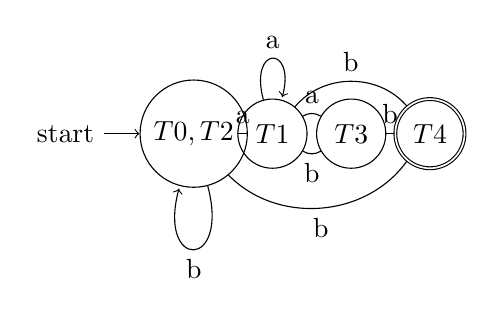
\begin{tikzpicture}
        \node[state, initial] (ac) {$T0,T2$};
        \node[state, right of=ac] (b) {$T1$};
        \node[state, right of=b] (d) {$T3$};
        \node[state, accepting, right of=d] (e) {$T4$};
	    \draw (ac) edge [loop below] node{b} (A)
	    (ac) edge [above] node{a} (b)
	    (b) edge [loop above] node{a} (b)
	    (b) edge [below, bend right=30] node{b} (d)
	    (d) edge [above, bend right=30] node{a} (b)
	    (d) edge [above] node{b} (e)
	    (e) edge [below, bend left=50] node{b} (ac)
	    (e) edge [above, bend right=50] node{b} (b)
	    ;
    \end{tikzpicture}
\end{document}
